\chapter{Introduction au modèle numérique}\label{ch:introduction}

Les echelles de temps sont radicalement opposées entre la cosmo qui considère les temps les plus long de l'univers et les progrès informatiques qui vont a une vitesse exponentielle. 
il faut considérer les simulations comme éphémère.

Comment modéliser la reionization?

\section{Les différents types de fluides cosmologique}

Un code de simulation cosmologique a pour vocation principale de suivre l'évolution de différents "fluides", comme la matière noire, la gaz, les étoiles, la radiation ou le champ magnétique.
Ces fluides sont de nature différentes et il n'y a pas de méthode permettant de suivre de manière optimale ces différentes physique.
On distinguera principalement deux catégories de fluides: les fluides collisionnels et les non-collisionnels.

\paragraph{Physique collisionnelle : } elle concerne principalement le gas.

\paragraph{Physique non-collisionnelle : } elle concerne principalement la matière noire ou les étoiles.



\section{Les différents types de codes}

Il existe conceptuellement deux principales façons de suivre un fluide dans l'espace.
Ces deux approches sont dites \emph{Eulérienne} ou \emph{Lagrangienne}.

\paragraph{Representation Lagrangienne : } 
consiste a se placer au point de vue du fluide.
On considère un élément de fluide pouvant se déplacer et/ou se dilater dans l'espace.
On associera généralement les codes utilisant ce type de représentation avec une gestion de la physique sous forme de \emph{particules}.

\paragraph{Representation Eulerrienne : } 
consiste a se placer au point de vue de l'espace.
On considère un élément d'espace et le bilan de matière entrant et sortant de chacune de ses interfaces.
On associera généralement les codes utilisant ce type de représentation avec une gestion de la physique sous forme de \emph{grille}.

EMMA utilise une représentation Lagrangienne pour simuler la matière noire et une représentation Eulerienne pour simuler le gas et la radiation.

En lien direct avec ces deux familles de représentation physique, il existe deux principales famille de codes cosmologique : les codes SPH et les codes AMR.



\paragraph{Smooth Particle Hydrodynamic (SPH) : } représente 

\paragraph{Adaptive Mesh Reffinement (AMR) :  }

%La représentation Lagrangienne la plus populaire (dans le domaine des simulations cosmologiques) est sans doute le \emph{Smouth Particle Hydrodynamics (SPH) }
%Les volumes cosmologiques étant généralement cubique, les éléments de grille le sont généralement aussi.



historique
avantage inconvénient AMR vs SPH
introduction de la grille et de la méthode AMR

\section{Gestion de la grille}
%(nécessaire d'être positionné ici car la structure en arbre conditionne plusieur choix par la suite)

Dans le cas des simulations sur grille fixe, les données sont réparties en mémoire de façon ordonnée.
Dans un espace en 3D, on accédera à une cellule contenant le point de coordonnées normées $(x,y,z)$ sur une grille de $N_x*N_y*N_z$ cellules, a l'aide de son identifiant Id dans le tableau en mémoire.

\begin{equation}
Id = i + j*N_x + k * N_x*N_y
\end{equation}
avec :
\begin{equation}
\begin{cases}
i=\lfloor x \rfloor *N_x \\
j=\lfloor y \rfloor*N_y \\
j=\lfloor z \rfloor*N_z \\
\end{cases}
\end{equation}
ou $\lfloor a \rfloor$ représente la partie entière de $a$.

Les choses sont plus complexes dans le cas d'une grille adaptative.

\begin{figure}[bth]
        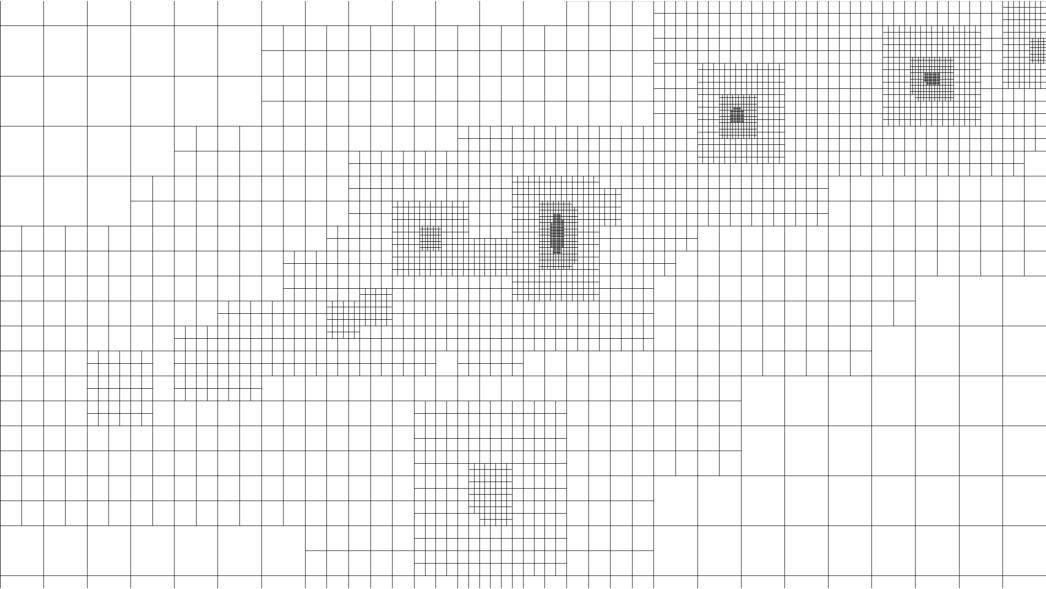
\includegraphics[width=.95\linewidth]{img/02/AMR.pdf} 
        \caption{AMR. 
}
 		\label{fig:AMR}
\end{figure}

\subsubsection{Octree}
fully threated tree description \citep{khokhlov_fully_1998-1}

Vu que la grille est amenées a évoluer, il n'est plus possible d'avoir une position unique en mémoire associé à une position dans l'espace.

La grille est composée de cellules non ordonnée.
Pour créer un lien entre elle, il est nécessaire de stocker l'information de voisinage.
cad que l'on a besoin de stocker 2*D pointeurs vers les cellules voisine.
 une cellule contient la partie physique 

Chaque cellule peut, sous certaine condition, etre subdivisée pour localement augmenter la résolution.
Elle devient alors asociée a un \emph{Oct} a 3 dimension.

Un oct est composé de 8 pointeurs vers ses 8 cellules filles, d'un pointeur vers sa cellule mère.

On associera également les octs entre eux a l'aide d'une liste chainée. 
Il est necessaire d'ajouter deux pointeurs a l'objet OCT : un vers l'oct précédent en mémoire et un vers l'oct suivant.


\begin{lstlisting}[float=bth,language=C,frame=tb,caption={les structures CELL et OCT de EMMA},label=lst:useless]
struct CELL{
  int id;            // permet de determiner la position de la cellule dans l'oct
  struct OCT *parent // l'oct pere de la cellule
  struct OCT *child; // si child est different de NULL alors la cellule est raffiner et child point vers l'oct enfant
  struct PHYSIC *data; // pointeur vers la partie physique
};

struct OCT{
  struct CELL cell[8]; // les 8 cellules de l'oct
  struct CELL *nei[6]; // pointeurs sur les cellule voisines
  struct CELL *parent; // cellule mere
  struct OCT *next;    // oct suivant dans la liste chainee
  struct OCT *prev;    // oct precedent dans la liste chainee
  int level;           // niveau de l'oct
};
\end{lstlisting}





\subsubsection{gestion du raffinement}
différentes condition de raffinement.\\
sur la matière noire\\
semi Lagrangienne\\
sur le gradient d'ionization\\
sur le gradient de densité (shock)\\





\subsubsection{Opérateurs de changement de grilles} \label{Opérateurs de changement de grilles}

La \emph{restriction} consiste à dégrader la grille en résolution. La restriction la plus directe consiste à moyenner les cellules à dégrader. Par exemple, sur une grille à deux dimensions, pour diviser la résolution par deux, quatre cellules de la grille de départ devront être moyennées pour obtenir une nouvelle cellule de la grille à base résolution. \\

La \emph{prolongation} consiste à augmenter la résolution d'une grille, la prolongation la plus directe consiste à injecter les valeurs de l'ancienne grille dans un certain nombre de cellules de la nouvelle grille. (fig \ref{Opérateurs de changement de grille})

\begin{figure}[htbp]
\begin{center}
\subfloat[Restriction]{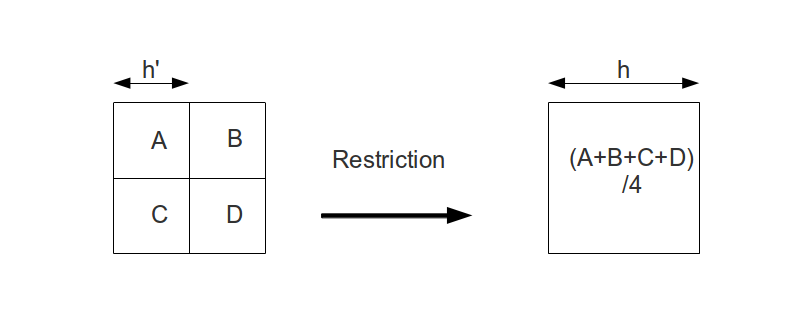
\includegraphics[scale=0.35]{img/02/Restriction.png}}
\subfloat[Prolongation]{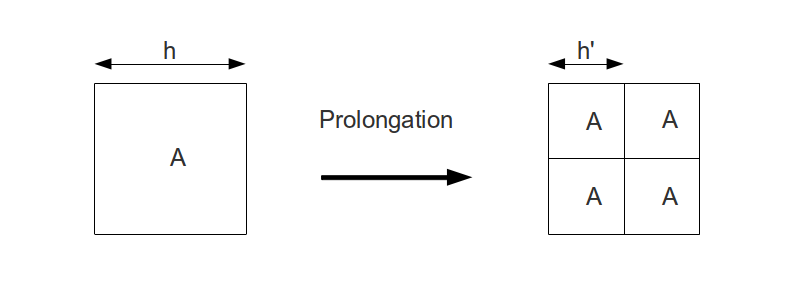
\includegraphics[scale=0.35]{img/02/Prolongation.png}}\\
\subfloat[Niveau L  ]{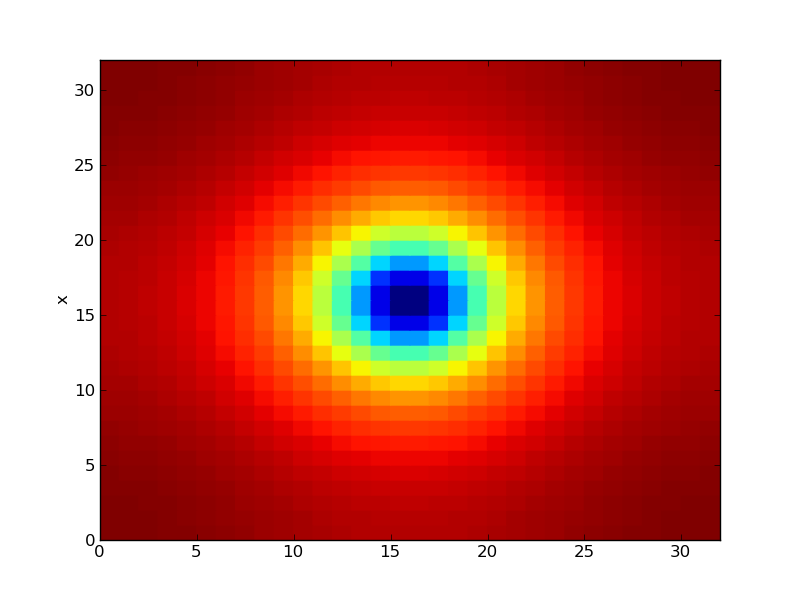
\includegraphics[scale=0.35]{img/02/0088.png} \label{Opérateurs de changement de grille c}}
\subfloat[Niveau L-1]{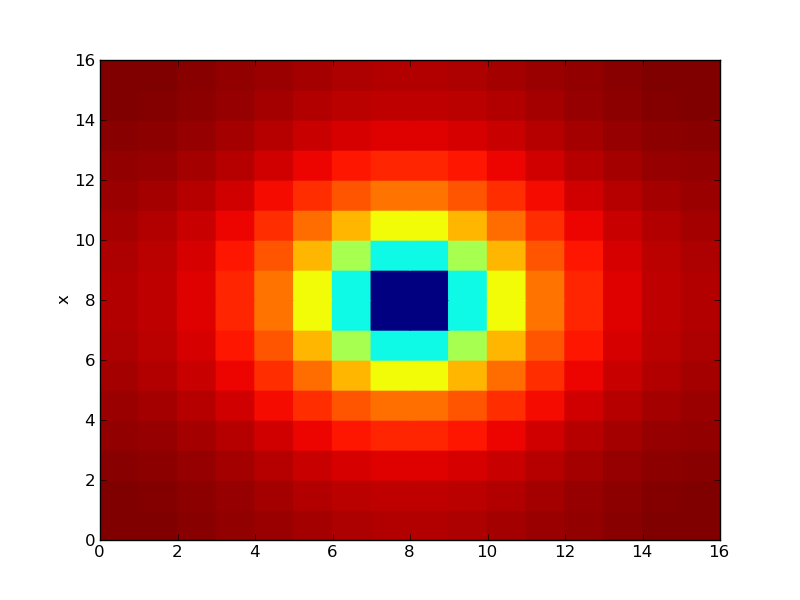
\includegraphics[scale=0.35]{img/02/0090.png} \label{Opérateurs de changement de grille d}}
\caption{\textbf{Opérateurs de changement de grille.} Ils permettent de changer la résolution de la grille. Un exemple de restriction consiste à moyenner une valeur de plusieurs cellules, la prolongation associée consiste en une injection directe d'une valeur dans plusieurs cellules.\\
Le potentiel du point masse prend une forme de losange à cause des conditions périodiques.}
\label{Opérateurs de changement de grille}
\end{center}
\end{figure}

La prolongation et la restriction sont des opérateurs aisément parallélisables. Chaque cellule (ou paquet de huit cellules) est indépendante des autres et il est possible de ne changer la résolution que d'une partie de la grille sans en affecter le reste.\\

Il existe principalement deux conditions sur les opérateurs de changement de grille. La première impose une certaine réciprocité entre eux, les opérateurs doivent être adjoints: il est nécessaire qu'après une prolongation, suivie d'une restriction la grille d'arrivée soit la même que la grille de départ. L'inverse n'est pas nécessairement vrai: après une restriction , de l'information est perdue et aucune prolongation ne pourra la recomposer. 
La seconde condition concerne la precision des opérateurs, il est nécessaire que la somme des ordres des opérations soit supérieure à l'ordre de l'équation à résoudre. Ici, la restriction est d'ordre trois, la prolongation d'ordre un et le Laplacien d'ordre deux, cette condition est vérifiée.



\section{Energie noire}
représente la majore partie du contenu de l'univers mais est la plus simple a simuler.
Lien direct avec le facteur d'expansion (mettre ref section).

Il existe deux possibilités pour modéliser l'expansion de l'univers.
La première consiste a considèrer un element de volume $dx$ de taille fixe, et au fur et a mesure que l'univers grandis, a y ajouter des élements.
Le problème et que le cout numérique de la simulation croit entre autre avec le nombre d'éléments que l'on considère.
La seconde possibilité est de faire varier la taille des éléments de calcul avec le facteur d'expansion.
On appellera les longueurs ainsi exprimées des longueurs comobile.

\begin{equation}
r=a r'
\end{equation}

ou $r$ représente une longueur en unités physique et $r'$ en unités comobile.

Ainsi un cube de 10 Mpc physique de coté, pris aujourd'hui, aura une taille de 10 Mpc comobile (cMpc) aujourd'hui, mais aussi a redshift z=9 ou sa taille physique ne sera plus que de de 1Mpc physique.

De plus, il est généralement pratique de normaliser les grandeurs que l'on considère. 

\begin{equation}
r'=\tilde{r}r*
\end{equation}
ou $\tilde{r}$ est la longueur normalisée et $r*$ le facteur de normalisation.


\subsection{Système d'unités supercomobiles}
La généralisation de ce principe a d'autre unités que la longueur est appeler système d'unités supercomobiles.
\citep{martel_convenient_1998}

Longueur:
\begin{equation}
\tilde{r}=\frac{r}{ar_*}
\end{equation}

Densité de matière:
\begin{equation}
\tilde{\rho}=\frac{\rho a^3}{\rho_*}
\end{equation}

Vitesse:
\begin{equation}
\tilde{v}=\frac{av}{v_*}
\end{equation}

Pas de temps:
\begin{equation}
\tilde{dt}=\frac{dt}{a^2t_*}
\end{equation}

Densité d'energie potentielle:
\begin{equation}
\tilde{\Phi}=\frac{a^2 \Phi}{\Phi_*}
\end{equation}

Pression:
\begin{equation}
\tilde{p}=\frac{a^5 p}{p_*}
\end{equation}

Densité d’énergie cinetique:
\begin{equation}
\tilde{\epsilon}=\frac{a^2 \epsilon}{\epsilon_*}
\end{equation}

Densité D’éléments:
\begin{equation}
\tilde{N}=a^3 N r_*^3
\end{equation}

Flux:
\begin{equation}
\tilde{F}=a^4 r_*^2 t_* F
\end{equation}



Facteurs de normalisation:
\begin{equation}
r_*=L (la taille de boite)
\end{equation}

\begin{equation}
\rho_* = \bar{\rho} = \frac{3H_0^2 \Omega_0}{8\pi G}
\end{equation}

\begin{equation}
t_* = \frac{2}{H_0 \sqrt{\Omega_m}}
\end{equation}

\begin{equation}
v_* = \frac{r_*}{t_*}
\end{equation}

\begin{equation}
\Phi_* = \frac{r_*^2}{t_*^2} = v_*^2
\end{equation}

\begin{equation}
p_* = \frac{\rho_* r_*^2}{t_*^2} = \rho_* v_*^2
\end{equation}

\begin{equation}
\epsilon_* = \frac{p_*}{\rho_*} = v_*^2
\end{equation}




\subsection{le pas de temps}

\section{Matière noire}
Ncorps

\subsection{génération des conditions initiales}

méthode
gaussian random noise
théorie des perturbation linéaire
lien avec le spectre de puissance
MUSIC et GRAPHIC
limite la résolution min et max (min en masse et max en espace)


une simulation est limité par sa taille et sa résolution -> ceci définit la plage d'échelle que l'on peut simuler

principes de bases ennoncé dans Pen (1997) and Bertschinger (2001).

    discrétisation de l'espace
    placement des particules sur la grille
    génération d'un bruit blanc
    convolution avec un spectre de puissance connu (celui du CMB)


\subsection{Théorie des perturbation linéaire}

approximation de zeldovich
perte de linéarité a un certain moment -> nécessité des simulation numériques





\subsection{solveur de gravité}
Le sloveur que je connais le mieux.

Fluide non collisionnel -> particule\\
On cherche a obtenir la position des particules a chaque instant -> il nous faut leurs vitesse -> il nous faut leurs accélération -> il nous faut la force qui leur est appliquée.
On peux obtenir cette force soit par calcul direct, soit par dérivation du potentiel.

\begin{equation}
\vec{F}=-\Delta \Phi
\end{equation}

le système d'équation de Vlasov-Poisson :

\begin{equation}
\begin{cases}

\frac{d{x}_p}{dt} = { v}_p, \\
\frac{d{ v}_p}{dt} = -\nabla \phi , \\
\Delta \phi= 4\pi G \rho.

\end{cases}
\label{eq:Ncorps}
\end{equation}


\paragraph{Particule-Particule : } c'est le méthode la plus directe pour calculer l'évolution d'un fluide non collisionnel. 
Elle consiste, pour chaque particule, a sommer les contribution gravitationnelles de toutes les autres particules.
Ce type de code dispose d'une très bonne précision mais la quantité de calcule évolue en ordre $O(N^2)$, ce qui fait que ce type de code est très coûteux.

\begin{equation}
\vec{F}_i=-\sum_{j\neq i} G \frac{G m_i m_j(\vec{r}_i - \vec{r}_j) }{ |\vec{r}_i - \vec{r}_j |^3}
\end{equation}

\paragraph{Particule-tree : } consiste a regrouper les particules loin de la particule courante en un amas aillant une interaction gravitationnelle commune
% (Barnes & Hut 1986) 

\paragraph{Particule-Mesh : } on projette les particules sur une grille
ENZO %code, Bryan & Norman 1998
RAMSES

La méthode de projection des particules sur la grille n'est pas unique.
On peut par exemple se contenter d'ajouter la masse de la particule dans la cellule a laquelle elle appartient.
Cela donne un résultat très bruité.
Une méthode d'ordre supérieure est appelé Cloud in cell (CIC)

\paragraph{Cloud in cell : } Le CIC consiste a considérer une étendue spatiale aux particules et a pondérée la masse appliqué au cellule par l'intersection de de son volume et de celui de la cellule.
Fig\,\ref{fig:CIC}.
On associe généralement une taille a la particule similaire a celle des cellule sur laquelle on la projette.
Dans le cas ou L’étendue de la particule intersecte des cellules de différents niveaux on lui associera la taille de la plus grande cellule dans le but de lisser la transition entre les niveaux.


\begin{figure}[bth]
        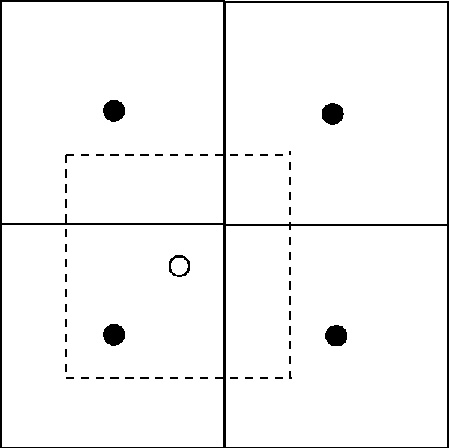
\includegraphics[width=.95\linewidth]{img/02/CIC.jpg} 
        \caption{Cloud In Cell. 
        %http://homepage.univie.ac.at/franz.vesely/cp_tut/nol2h/new/c6sm_s4lr.html
}
 		\label{fig:CIC}
\end{figure}

Il existe des méthodes d'ordre supérieur avec des kernel plus complex que le top-hat du CIC comme par exemple des kernel en triangle ou en gausienne.
%http://techfinder.stanford.edu/technology_detail.php?ID=30866

Une fois la grille de densité générée nous pouvons calculer le potentiel.

\subsubsection{l'équation de Poisson}
\begin{equation}
\Delta \Phi = 4 \pi G \rho
\end{equation}

qui devient en système d'unité supercomobile:
\begin{equation}
\Delta \Phi = 6 a \delta
\end{equation}
avec le contraste de densité: 
\begin{equation}
\delta = \tilde{\rho} / < \tilde{\rho} > - 1 
\end{equation}

integration de l'equation de Poisson pour obtenir le potentiel
\begin{equation}
\Delta \phi = 4\pi G \rho \longrightarrow \phi = \iint \Delta \phi = \iint 4\pi G \rho
\end{equation}

Pour cela, il existe principalement deux types de méthodes. La première est basée sur les Transformées de Fourier. Cette méthode, très rapide, utilise le fait que dans l'espace de Fourier, une intégrale se résume à une division par un nombre d'onde. Déterminer le champ de potentiel revient à : 
\begin{itemize}
\item Effectuer la transformée de Fourier de la densité
\item Diviser par $k^2$
\item Effectuer la transformée de Fourier inverse
\end{itemize}

\begin{equation}
\rho_{(\vec{x})} \overset{FFT}{\longrightarrow}  \rho_{(\vec{k})} \times \frac{1}{k^2}  \overset{RFFT}{\longrightarrow}  \phi_{(\vec{x})}
\end{equation}

De par la nature des transformées de Fourier, le champ de densité doit être périodique pour que l'implémentation de cette technique ne se révèle pas trop complexe. Ce qui n'est pas un problème en simulation cosmologique, où les conditions de bords sont toujours périodiques mais est plus problématique lors de la simulation de structures isolées, telles les galaxies ou les amas de galaxies. Ensuite, les FFT nécessitent un échantillonnage régulier ce qui implique que cette méthode est incompatible avec les grilles adaptatives. Et dernièrement, le passage dans l'espace des fréquences nécessite des conditions de types plans parallèles lors parallélisation, conditions incompatible avec la gestion de grille utilisé par les code AMR dont \emph{Quartz} fait partie. \\

Un autre type de méthode de résolution possible est une méthode itérative. Elle consiste à faire converger le potentiel à partir d'une condition initiale arbitraire. Ce type de méthode est plus lente que la méthode par FFT mais  permet d'utiliser tout type de conditions de bords, d'être facilement parallélisable et surtout est compatible avec les méthodes basées sur des grilles adaptatives. PAr la suite, c'est donc une méthode itérative et plus précisément une méthode \emph{Multigrille} qui à été développée.\\

Le potentiel est alors dérivé pour obtenir la force ressentie dans chaque cellule. Il est ensuite aisé de calculer l'accélération subie par les particules de chaque cellule, et par intégration temporelle, leurs nouvelles positions et vitesses.

Par analogie à l'équation de la chaleur par exemple, la densité correspond aux sources chaudes et le potentiel à la température, à $t=0$ les sources chaudes sont allumées et la chaleur se propage jusqu'a ce que le milieu ait atteint sa température d'équilibre. Ici, c'est donc la gravité qui se diffuse dans le milieu. \\


\begin{equation}
\dfrac{\partial \phi}{\partial t} = \Delta \Phi -S 
\end{equation}


\subsubsection{Méthode jacobi}


La méthode de Jacobi est la façon la plus simple de relaxer ce type d'équation, elle consiste à utiliser directement la forme discrète de l'équation de Poisson modifiée. L'équation à intégrer est:

\[ \dfrac{\phi^{t+1}_i - \phi^{t}_i}{\Delta t}  =  \Delta \phi_i^t - 4 \pi G \rho^t_i \]

où, à 3 dimensions, le Laplacien s'exprime :

\[ \Delta \phi_i^t = \dfrac{\phi_{x+1,y,z}^t  + \phi_{x-1,y,z}^t + \phi_{x,y+1,z}^t  + \phi_{x,y-1,z}^t + \phi_{x,y,z+1}^t + \phi_{x,y,z-1}^t	- 6\phi_{x,y,z}^t}{\Delta x ^2} \]
		
Le principal avantage de cette méthode est sa parallélisation triviale. 
Elle ne nécessite de connaître l'état du système qu'au temps $t$. 
Ansi, chaque fils d'exécution parallèle (thread) est indépendant et n'a pas d'information à communiquer aux autres .



\subsubsection{Gauss Seidel}
Gauss-Seidel est une amélioration de Jacobi. Au lieu d'utiliser, à chaque pas de temps, les valeurs de la grille au niveau précédent, cette méthode consiste à toujours utiliser la valeur la plus à jour disponible. Une fois $\phi^{t+1}_0$ calculé à l'aide de $\phi^{t}_i$, la valeur de $\phi^{t+1}_1$ n'est pas calculée à l'aide de $\phi^{t}_0$ mais avec $\phi^{t+1}_0$. En utilisant toujours la valeur la mieux estimée, cette méthode accélère la convergence. L'intégration temporelle ne change pas, mais l'intégration spatiale devient: 

\[ \Delta \phi_i^t = \dfrac{\phi_{x+1,y,z}^t  + \phi_{x-1,y,z}^\mathbf{t+1} + \phi_{x,y+1,z}^t  + \phi_{x,y-1,z}^\mathbf{t+1} + \phi_{x,y,z+1}^t + \phi_{x,y,z-1}^\mathbf{t+1}	- 6\phi_{x,y,z}^t}{\Delta x ^2} \]

La parallélisation de cette méthode est plus compliquée que dans le cas de Jacobi. La détermination de la valeur de chaque cellule nécessite de connaître l'état le plus à jour de ses voisins et donc de faire passer de l'information entre les threads.
 Cependant, une méthode nommée Gauss-Seidel Rouge-Noir permet une parallélisation sur multiprocesseurs en séparant l'espace en un damier de couleurs. Chaque processeur ne calcule alors qu'une seule couleur. Le premier processeur calcul par exemple les cases blanches de l'échiquier à partir de $\phi_i^t$, puis le second calcul le cases noires à partir des cases blanches déterminé par le premier.


\subsubsection{Sur-relaxation successive (SOR)}
La méthode de sur-relaxation successive consiste à appliquer un coefficient à la méthode de Gauss-Seidel (ou de Jacobi, en fonction de la méthode de dérivation spatiale) pour sur-estimer l'évolution de la convergence et ainsi l'accélérer. l'équation à intégrer devient:
\[ \phi^{t+1}_i = \phi^{t}_i + \omega  \Delta t \left (\Delta \phi_i^t - 4 \pi G \rho^t_i \right )  \]
où $\omega \in \left] 0,2 \right [$ est le paramètre de sur-relaxation.
\begin{itemize}
\item lorsque $\omega <1$ La méthode est dite de sous relaxation.
\item lorsque $\omega =1$ La méthode devient celle de Gauss-Seidel.
\item lorsque $\omega >1$ La méthode est dite de sur relaxation.
\end{itemize}
Il existe des moyens analytiques pour déterminer la valeur optimale de $\omega$ mais très souvent cette valeur est déterminée empiriquement à partir d'une série de tests. $\omega = 1,2$ est très souvent utilisé.
%L'expression de cette méthode apparait généralement dans la litterature sous la forme:


\subsubsection{Condition d'arrêt}
Ces méthodes sont itérées jusqu’à ce qu'un certain critère convergence soit respecté. Le critère le plus couramment utilisé consiste à mesurer l'évolution de la convergence en comparant sa valeur au temps $t$ à celle au temps $t+1$.
\[ \phi^{t+1}_i - \phi^{t}_i < \epsilon \]
ou, de manière équivalente:
\[ \Delta \phi_i^t - 4 \pi G \rho^t_i< \epsilon \]

Pour prendre en compte la possibilité que le potentiel ait convergé sur une partie du domaine seulement, et pour ne pas stopper le processus trop tôt, c'est le module de cette expression qui est considéré. De plus il est d'usage de normaliser ce module par la source que l'on considère.

\[\dfrac{ \sqrt{  \sum_i \left (  \Delta \phi_i^t \right )^2 - \left (4 \pi G \rho^t_i  \right )^2 } }{\sqrt{  \sum_i  \left (4 \pi G \rho^t_i  \right )^2 } } < \epsilon \]

A cette condition est ajouté un nombre d'itérations maximum fixe pour éviter les problèmes de boucles infinies lorsque le potentiel n'arrive pas à converger (oscillation autour d'une valeur d'équilibre par exemple).

\subsubsection{Multigrille}
Cette seconde technique, plus efficace encore, consiste à travailler non pas sur la grandeur elle même, mais sur l'erreur effectuée dans l'estimation de cette grandeur.

Elle utilise la linéarité de l'opérateur Laplacien: 
 
Si l'équation à résoudre est de la forme : 
\[ \mathcal{L} u = f \]
Sa forme discrète est :
\[ \mathcal{L}_h u_h = f_h \]
si $\tilde{u_h}$ correspond à une estimation de la solution et $u_h$ à la solution exacte, l'erreur est alors la différence entre les deux : 
\[ v_h = u_h - \tilde{u_h} \]
le résidu est défini comme:
\[ d_h = \mathcal{L}_h \tilde{u_h} - f_h \]
comme $\mathcal{L}_h$ est linéaire:
\[ \mathcal{L}_h u_h = \mathcal{L}_h (v_h + \tilde{u_h} ) = \mathcal{L}_h v_h +\mathcal{L}_h \tilde{u_h} \]
\[ f_h   = \mathcal{L}_h \tilde{u_h} - d_h\]
et finalement :
\[ \mathcal{L}_h v_h = -d_h \]

L'équation à résoudre est alors modifiée en considérant que l'inconnue n'est plus le potentiel mais l'erreur commise sur son estimation. Le terme source n'est plus la densité mais la densité moins son estimation grossière.\\


Le cycle consiste à lisser (relaxer quelques fois) le potentiel à pleine résolution, les petites échelles vont alors rapidement converger, à calculer ensuite l'erreur commise à ce stade. L'erreur est dégradée à plus basse résolution, elle ne contient alors que de l'information sur les basses fréquences de la grille de départ, les hautes fréquences de la grille à pleine résolution ont été supprimées par la dégradation. Cette perte d'information sur les hautes fréquences n'est pas problématique car les hautes fréquences ont déjà convergé l'erreur est donc petite (voir nulle) aux hautes fréquence et est maximale aux basses. Les hautes fréquences de cette nouvelle grille correspondent alors à des fréquences plus basses et donc plus difficiles à faire converger sur le grille globale. La solution exacte de l'équation de l'erreur est calculée par itération (relaxée jusqu'a convergence) à partir des résidus sur cette petite grille. Le potentiel précédemment estimé est alors corrigé de l'erreur exacte interpolée à pleine résolution en utilisant:
\[ \tilde{u}_h^{new} = \tilde{u_h} + v_h \]
Le potentiel corrigé est alors lissé par quelques dernières itérations.\\

Ce cycle peut être résumé ainsi:


\begin{tabular}{ll}
Lisser 		& 	$ \mathcal{L} u_h = f_h $\\
Calculer	&	$ d_h = \mathcal{L}_h \tilde{u_h} - f_h $\\
Restreindre	&	$ d_H = Rd_h$\\
Résoudre	&	$ \mathcal{L} v_H = -d_H $\\
Interpoler	&	$ v_h = Pv_H$\\
Corriger	&	$ \tilde{u}_h^{new} = \tilde{u_h} + v_h$\\
Lisser		&	$ \mathcal{L} u_h = f_h $
\end{tabular} 



A partir de la méthode deux grilles, rien n'empêche d'estimer l'erreur sur l'erreur par la même méthode, ce processus peut être utilisé récursivement pour générer tout un ensemble de sous grilles et ainsi accélérer encore la convergence.\\

L'algorithme devient alors:\\

MG(level, $u_h$, $f_h$)
\begin{itemize}	
\item 	si level = level min:
\item[]	\begin{tabular}{ll}
		Résoudre & $\mathcal{L} u_h = f_h $
		\end{tabular}
\item 	sinon:
\item[]	\begin{tabular}{ll}
		Lisser 		& 	$ \mathcal{L} u_h = f_h $\\
		Calculer	&	$ d_h = \mathcal{L}_h \tilde{u_h} - f_h $\\
		Restreindre	&	$ d_H = Rd_h$\\
		Appeler 	&	MG(level-1, $v_H$, $-d_H$) \\
		Interpoler	&	$ v_h = Pv_H$\\
		Corriger	&	$ \tilde{u}_h^{new} = \tilde{u_h} + v_h$\\
		Lisser		&	$ \mathcal{L} u_h = f_h $
		\end{tabular} 
\end{itemize}

Où la taille de la grille au niveau "level" est de $2^{3level}$ ( si level = 9, la taille de la grille est de $512^3$ ). $h$ est le pas de la grille au niveau "level" et $H = 2h$. Les opérateurs $P$ et $R$ sont les opérateurs de prolongation et de restriction explicité section \ref{Opérateurs de changement de grilles}
Cet algorithme est représenté graphiquement sur la figure \ref{Description du V-cycle}.


\begin{figure}[htbp]
\begin{center}
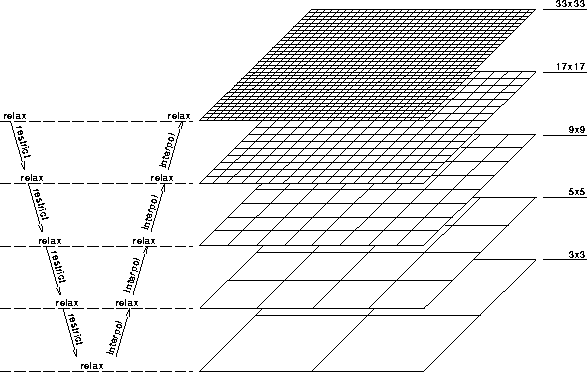
\includegraphics[scale=0.35]{img/02/multigrid.png}
\caption{\textbf{Vue des différents niveaux de grilles.} Image extraite de \href{http://MGNet.org}{MGNet.org} }
\label{Vue des différents niveaux de grilles}
\end{center}
\end{figure}	

\begin{figure}[htbp]
\begin{center}
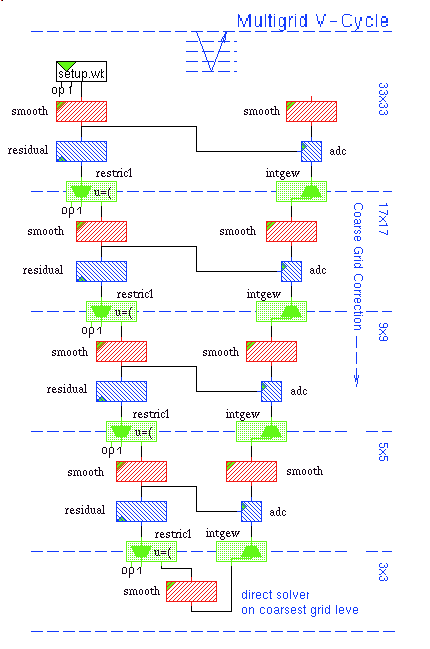
\includegraphics[scale=0.35]{img/02/Vcycle.png}
\caption{\textbf{Description du V-cycle.} Image extraite de \href{http://MGNet.org}{MGNet.org}}
\label{Description du V-cycle}
\end{center}
\end{figure}		

En jouant sur le nombre d'appels récursifs de la fonction, il est possible de créer différentes géométries de cycles. Un seul appel génère un cycle nommé cycle en V (fig. \ref{Description du V-cycle}), deux un cycle en W, etc... 

			



le pas de temps\\

\section{Baryon}

système d'équations a résoudres

\begin{equation}
\begin{cases}

{ \frac{ \partial \rho }{ \partial t } + \nabla \cdot (\rho v) = 0}, \\
\\
{ \frac{ \partial }{ \partial t } (\rho v) + \nabla \cdot (\rho v \otimes v ) \nabla p = -\rho\nabla \phi }, \\
\\
{ \frac{ \partial e }{ \partial t } + \nabla \cdot [ \rho v (e+p/\rho) ] = -\rho v \cdot \nabla \phi },

\end{cases}
\end{equation}
\label{eq:hydro}



solveur hydro
partie la plus intensive en calcul
le pas de temps

\section{La chimie}

gestion du refroidissement

\section{radiation}

\subsection{Les equations}
\begin{equation}
\frac{1}{c} \frac{\partial I_\nu}{\partial t} + \vec{n}\cdot \vec{\nabla} I_\nu = \eta_\nu - \kappa_\nu I_\nu 
\end{equation}
Avec: $I_\nu(\vec{x},\vec{n},t)$ l'intensité spécifique
$\eta_\nu(\vec{x},\vec{n},t)$ la source de rayonnement

et le coefficient d'absorption $\kappa_\nu(\vec{x},\vec{n},t) = \sigma_\nu n_H$ 
$\sigma_\nu$ la section efficace de photoionisation de l'H neutre et $n_H$ la densité d'H neutre


\begin{equation}
\begin{cases}

\frac{ \partial N_\nu }{ \partial t } + \vec{\nabla} \cdot \vec{F}_\nu = -\kappa_\nu c  N_\nu + S_\nu,\\

\frac{ \partial \vec{F} }{ \partial t } + c^2 \vec{\nabla} P_\nu = -\kappa_\nu c \vec{F}_\nu ,

\end{cases}
\label{eq:densite_energie}
\end{equation}

$\vec{F}_\nu$ le flux radiatif

$P_\nu $ la pression radiative

et 

$S_\nu = \dot{N}_\nu^* + \dot{N}_\nu^{rec}$ etant le taux d'emission de photon due aux sources $\dot{N}_\nu^*$ et a la recombinaison $ \dot{N}_\nu^{rec}$


\subsection{approximation M1}
La fermeture du système se fait par l’intermédiaire de l’équation
d’état, avec le tenseur d’Eddington, D :

\begin{equation}
 P_\nu = D N\nu ,
\label{eq:fermeture}
\end{equation}

où D est approximé par le modèle M1 \citep{levermore1984,gonzalez2005} :

\begin{equation}
\begin{cases}

D = \frac{ 3\chi -1 }{2} \mathbb{1} + \frac{ 1 - \chi }{2} \vec{n} \otimes \vec{n} , \\
\\
\chi(\vec{f}_\nu) = \frac{ 3+4 |\vec{f}_\nu|^2 }{5+2\sqrt{4-3|\vec{f}_\nu|^2}} , \\
\\
\vec{f}_\nu = \frac{ \vec{F}_\nu }{c N\nu }  ,

\end{cases}
\label{eq:tenseur}
\end{equation}


\subsection{discretisation}
\begin{equation}
\rm{ \frac{\partial U}{\partial t} + \nabla \cdot (F(U)) = S(U), }
\label{eq:rad_generale}
\end{equation}

avec $\rm{U}$ le vecteur des quantité conservées, $\rm{F}$ la fonction de flux, et $\rm{S}$ le terme source. Pour la résolution du transport des photons (sans terme source), on retrouve :

\begin{equation}
\rm{ \frac{ U^{p+1}_i - U^{p}_i }{\Delta t} + \frac{ F^{p}_{i
+1/2} - F^{p}_{i-1/2} }{\Delta x} =0,}
\label{eq:rad_solver}
\end{equation}

Condition de Courant radiative : $\rm{ c \leq \Delta x / \Delta t }$.
Le pas de temps est donc plusieurs ordres de grandeur plus petit que celui de l'hydrodynamique.

\subsection{vitesse de la lumière reduite}


système d'équations a résoudre
la méthode M1
aton
le cooling
le pas de temps
la mise en place du multi longueur d'onde

\section{gestion du pas de temps}

condition de courant
cosmo
part
freefall
hydro
radiatif

\section{Matérie et parallélismel}

Les simulations cosmologiques ont pour principal defi de simuler d'important volume d'espace avec la meilleure résolution possible.
L'amelioration de certain algorythme a permis d'augmenter la taille des simulations mais le principal facteur limitant se trouve au niveau du materiel.
Dans le but d'augmenter la puissance de calcul, les machines se regroupent en centre de calcul.

Ces machines se composent d'un certain nombre de nœuds.

\paragraph{Nœud :} Élément du centre de calcul relier par un réseau.
Proche d'un ordinateur personnel il est composé d'une carte mère sur laquelle est relié entre autres, un ou plusieurs processeurs (CPU), une certaine quantité de mémoire RAM et parfois une carte graphique (GPU)

Chaque CPU dispose d'un certain nombre de cœurs, et chaque cœurs est capable d'exécuter un certain nombre de processus ou thread (généralement 1, et parfois 2 dans le cas de l'Hyperthreading)

La difficulté est de géré la façon dont les threads travaillent ensemble.
En effet a chaque thread sera associé un domaine de calcul représentant une partie de l'espace a modeliser.
De plus les domaine ne sont pas isolés et partage de l'information. 

Nous sommes alors confronté a plusieurs problèmes: comment associer les threads aux domaines de calculs  et comment faire communiquer ces threads entre eux.

\subsection{courbe de Peano-Hilbert}

%https://books.google.fr/books?id=sbQqBgAAQBAJ&pg=PA26&lpg=PA26&dq=peano+hilbert+mpi&source=bl&ots=HgSw0Jpf7d&sig=vXTb2JkDixd1gcDGANoARIYHAG0&hl=fr&sa=X&ved=0ahUKEwilofzKoerSAhUF6RQKHXzQDC4Q6AEIGjAA#v=onepage&q=peano%20hilbert%20mpi&f=false


%Warren et Salmon
Le découpage des domaines de calcul correspondants aux différents processeurs,  utilise une courbe de Peano-Hilbert.
Ce type de courbes fractale a la particularité de remplir l'espace.
Mais aussi de passer par tout les points d'une grille.
Ainsi si l'on applique ce pavage aux cellules de notre grille, en associant un indice reliant un cellule a sa position sur la courbe de Hilbert.
Il suffit ensuite de découper la courbe en parties identique  pour 
Ainsi si l'on a par exemple  32 cellules a assigner sur 4 processeurs, la courbes sera découpée en 4 parties de 8 cellules.
Chacune de ces partie sera en suite assignée a un processeur.

Ce type de découpage minimise les interfaces entre domaine, en s'assurant d'une proximité spatiale entre tout les points de la courbe.
Elle minimise donc les communications entre processeurs

\begin{figure}[bth]
        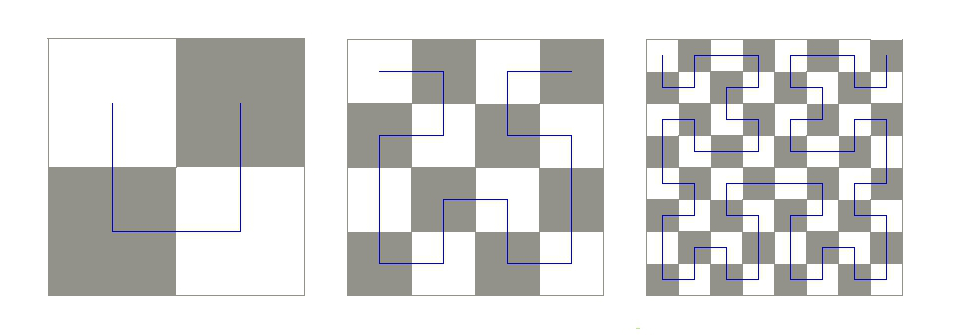
\includegraphics[width=.95\linewidth]{img/02/courbe_Hilbert.jpeg} 
        \caption{exemple de courbe de Hilbert. 
        %http://www.lifl.fr/~pmathieu/transform/fractales.html
}
 		\label{fig:hilbert}
\end{figure}


\begin{figure}[bth]
        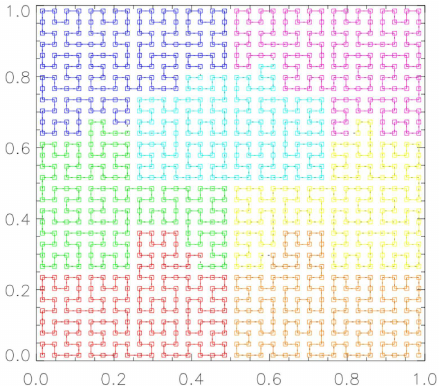
\includegraphics[width=.95\linewidth]{img/02/hilbert2.png} 
        \caption{exemple de courbe de Hilbert. 
%http://iopscience.iop.org/article/10.1086/590370/pdf 
}
 		\label{fig:hilbert2}
\end{figure}


\subsection{Mémoire partagée et mémoire distribuée}

Une fois les processus et les domaines identifiés il existe différentes facons de faire dialoguer les processus entre eux.
La principale distinction viendra généralement de si les threads sont exécutés par un meme noeud ou non.

\paragraph{mémoire partagée : } 
Si les threads sont éxécutés sur un meme noeud on aura tendance a utiliser un schéma a base de mémoire partagée.
On dit que la mémoire est partagée quand plusieurs threads ont accès au meme espace memoire, cad par exemple que si le thread 0 déclare une variable X, le thread 1 aura aussi accès a cette variable . 
OpenMP est une API permettant ce  genre partage de mémoire.

\paragraph{mémoire distribuée : } 
Dans le cas ou les threads sont exécutés par des processeurs étant physiquement éloigné, ie sur des noeuds différents, les communications doivent passer par un réseau de communication reliant les noeuds.
Il faudra utiliser dans ce cas une autre API pour explicitement envoyer et recevoir des paquets d'information
L'API la plus communément utilisée pour ce genre de communication est Message Passing Interface MPI.


%Je n'ai aucun doute sur le fait que dans les années a venir 


\subsection{GPGPU}

Les cartes graphiques, ou GPU ont été détourné de leurs utilisation principale d'affichage il y a une dizaine d'années.
Ces unités de calculs sont  efficaces dans le traitement d'un grand nombre d'information en parallèle.
Elle sont donc toutes indiqué dans le cas des simulation numérique.

La programmation sur carte graphique utilise une approche proche du concept de mémoire distribuée.
Cad que la carte graphique GPU et le processeur central CPU ont besoin de communiquer.

Or a l'heure actuelle cette communication utilise une interface relativement lente (PCI express) qui rend couteuse la communication. 
Il faut donc que la quantité de calcul effectués par la carte soit suffisante pour rentabilisé la communication.





\subsection{Gestion des entrées sortie}

le feedback CODA\\
grosse quantité de données\\

L'objectif durant ma thèse était de réaliser une simulation de la reionization avec un nombre de particule de matière noire (et donc une grille coarse) de 2048**3.
Et si il faut calculer ces données, il faut également les stocker, cad les écrire sur disque dur.

\begin{itemize}

\item Pour les particule:
en considerant qu'un flottant est codé sur 8 bits, chaque champs represente 8Go.
Il y a une dizaine de champs en sortie (3 positions, 3 vitesses, etc): environs 80Go

\item Pour la grille :
En considérant qu'approximativement la quantité de cellule est multipliée pas 3 a cause du raffinement  chaque champ physique (densité, température, composante de la vitesse, etc..) représente environ 24Go de donnée.
Il y a au total un cinquantaine de champs physique nécessaire a l'exécution de la simulation mais en pratique environ une vingtaine en sortie.
Chaque écriture représente donc 500Go pour la grille.

\item Pour les étoiles:
c'est très variable car dépend directement du nombre d'étoile a l'instant donné, qui dépend lui même du paramètre de résolution.

\end{itemize}

Soit au total envrion 600Go par instant.

Mais on voudrait évidemment avoir accès a l'état de la simulation a différents instant.
Cette simulation a généré 170 snapshot.
Au final le volume de donnée de la simulation représente environs une centaine de tera octets.

Les entrées sorties sont des etapes relativement longues et l'ecriture sur disque d'une telle quantité de données demande du temps et ralentit l'exécution de la simulation.
De plus, ces données sont généralement calculé sur des machines distante et leurs rapatriement sur des machine locales peut également être couteux en temps (parfois plusieurs mois)
%analyse a distance

Architecture des données 

conception d'une organisation des données
séparation des champs
structure imposé par la gestion de l'AMR
utilisation de hdf5
écriture parallèle

%\subsection{Potentiel d'optimisation EMMA}
%
%la forme des gathers/scatter
%optimisation matérielle -> les prochaines générations de GPU
%Opérations coarse sur grille non AMR.
%reformatage de l'arbre et découplage de la physique
